\chapter{Forforstærker}
\label{forforstaerker}
Forforstærkerens opgave er, som nævnt i kapitel \ref{systemopbygning}, at forstærke et mikrofonsignal op til linieniveau. Ved gennemgangen af relevante standarder i afsnit \ref{standarder} ses det, at et liniesignal ligger med peakspændinger mellem 200 mV og 2 V, mens et mikrofonsignal ligger med peakspændinger mellem 0,8 mV og 200 mV. Der er altså for et liniesignal en faktor 10 mellem den laveste og den højeste signalspænding, mens der for et mikrofonsignal er en faktor 250 mellem de to yderpunkter. Denne forskel bevirker at signalet fra en mikrofon, hvis udgangssignal ligger i området beskrevet i standarden, ikke kan forstærkes lineært til linieniveau.\\ 
Forforstærkeren bliver derfor designet til én bestemt type mikrofon, som var let tilgængelig for gruppen, nemlig en Monacor MCE-4000 \fixme{kilde: mce-4000.pdf}. Denne mikrofons udgangsspænding er givet i databladet ved en følsomhed på $5~mV/Pa$. For at fastsætte et forventeligt arbejdsområde tages der udgangspunkt i at almindelig tale foregår ved $60~dB(A)$\fixme{kilde: http://www.es.aau.dk/sections/acoustics/press/fakta/lidt\_om\_lyd/}. Givet at spændingen efter forforstærkeren må variere med en faktor 10 og forforstærkeren ønskes at forstærke lineært, må spændingen ind i forforstærkeren også kun variere med en faktor 10. Da $dB(A)$ er en logaritmisk skala, må lydtrykket i mikrofonen altså variere med $20~dB(A)$. Arbejdsområdet vælges sådan, at lydtrykket for almindelig tale ligger midt i, hvormed arbejdsområdet bliver fra $50~dB(A)$ til $70~dB(A)$. Disse grænser omregnes ved brug af formel (\ref{equ:db-pa}), hvor $p_{ref} = 20~\mu Pa$ og $L_p$  er henholdsvis $50~dB(A)$ og $70~dB(A)$. 

\begin{equation}
\label{equ:db-pa}
p_{min} = 10^{\frac{L_p}{20}} \cdot p_{ref}
\end{equation}

Grænseværdierne bliver dermed $6,3~mPa$ og $63~mPa$. Yderpunkterne i peakspændingen forforstærkeren skal håndtere kan dermed bestemmes ved hjælp af formel (\ref{equ:vmicpeak}), hvor $p$ sættes til henholdsvis $6,3~mPa$ og $63~mPa$.

\begin{equation}
\label{equ:vmicpeak}
\hat{V}_{microphone} = p \cdot 5\frac{mV}{Pa}
\end{equation}

Peakspændingerne bliver dermed $\hat{V}_{min} = 31,5~\mu V$ og $\hat{V}_{max} = 315~\mu V$. Med disse spændinger på plads ses det at forforstærkeren skal forstærke 6350 gange for at få det op på liniesignalsniveau. De samlede krav til forforstærkeren er vist i tabel \ref{tab:krav_forforstaerker}

\begin{table}[h]
\centering
\begin{tabular}{l|r}
\hline\hline
Område & Krav \\
\hline\hline
Forstærkning & 6350 gange \\[4pt]
Forvrængning & < 0,5 \% \\[4pt]
Indgangsimpedans & > 5 k\ohm \\
\hline\hline
\end{tabular}
\caption{Krav til forforstærkeren}
\label{tab:krav_forforstaerker}
\end{table}

\section{Design}

\begin{figure}[h]
\centering
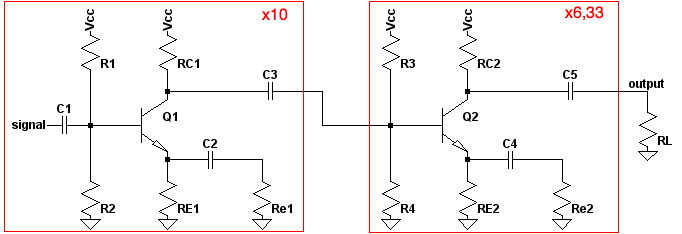
\includegraphics[scale=.6]{teknisk/forforstaerker/blok_forforstaerker.png}
\caption{Blokdiagram over forforstærkerens byggeblokke samt lydsignalets vej}
\label{blok_forforstaerker}
\end{figure}

Udregningerne kan ses i vedlagt pdf (beregning-forforstaerker.pdf). 


\section{Simulering}


\section{Accepttest}

